\documentclass{jsarticle}
\title{講義ノート第6回}
\author{}
\date{}


\usepackage[top=30truemm,bottom=30truemm,left=25truemm,right=25truemm]{geometry}

\usepackage{ascmac}

\usepackage{amsmath}

\usepackage[dvips]{graphicx}

\usepackage{ulem}

\parindent = 0pt

\begin{document}
\maketitle

\section{静電場}

\setcounter{subsection}{10}

\subsection{静電ポテンシャル}

ここまで,Coulombの法則から出発し静電場の性質がいくつか分かった.その一部が
\begin{equation*}
{\rm div}{\bf E}=\frac{\rho}{\varepsilon_0} , {\bf E} = - {\rm grad}{\phi}
\end{equation*}
である. \\
2つの性質は,{\bf Poisson方程式} によって1つにまとめられる. \\
2式から電場${\bf E}$を消すと,
\begin{eqnarray*}
{\rm div}({\rm grad} \phi) = - \frac{\rho}{\varepsilon_0}
\end{eqnarray*}
\begin{eqnarray*}
\mbox{左辺} &=& \frac{\partial}{\partial x}({\rm grad} \phi)_x + \frac{\partial}{\partial y}({\rm grad} \phi)_y + \frac{\partial}{\partial z}({\rm grad} \phi)_z \\
&=& \left( \frac{\partial^2}{\partial x^2} + \frac{\partial^2}{\partial y^2} + \frac{\partial^2}{\partial z^2} \right) \phi
\end{eqnarray*}
ここで微分演算子Laplacianを以下のように定義する.
\begin{eqnarray*}
\bigtriangleup = \frac{\partial^2}{\partial x^2} + \frac{\partial^2}{\partial y^2} + \frac{\partial^2}{\partial z^2}
\end{eqnarray*}
すると以下のPoisson方程式が得られる.
\begin{itembox}[c]{Poisson方程式}
\begin{eqnarray}
\bigtriangleup \phi = - \frac{\rho}{\varepsilon_0}
\end{eqnarray}
\end{itembox}
これは静電場の法則を集約した式であるから,静電場の問題はこのPoisson方程式の解を求めることに集約される.\\
また,Poisson方程式の重要な性質として,電荷密度$\rho$と境界条件が指定されると解が一意的である,というものがある.境界条件とは境界における$\phi$の値,あるいは${\rm grad}\phi$の法線成分の値のことである. \\
{\bf 例} \\
ある閉曲面があり,その内部は電荷が全く無く空洞であり,境界で等電位であるとする.内部空洞の電場${\bf E}$を求めたい. \\
そのためにまずPoisson方程式から,空洞における電位$\phi$を求める. \\
内部ではいたるところ電荷が存在しないから,電荷密度$\rho$は0である.したがってPoisson方程式は, $\bigtriangleup \phi = 0$ \\
ここで境界条件を考えると,境界では電位は一定値$\phi_0$をとる.したがって$\phi({\bf e}) = \phi_0$としてみると,これはPoisson方程式を満たす. \\
したがってこれが解であり(解の一意性)空洞内部から境界まで至るところ等電位であることがわかる. \\
求める電場は,${\bf E} = - {\rm grad} \phi_0 = 0$ である.

\subsection{静電エネルギー}
2体間の静電エネルギー$U_{12}$を無限遠を基準として以下のように定義する.
\begin{eqnarray*}
U_{12} = \frac{q_1q_2}{4 \pi \varepsilon_0 |{\bf r}_1-{\bf r}_2|}
\end{eqnarray*}
するとn体の静電エネルギー$E$は,全ての電荷が十分離れている状態を基準として以下のように書ける.
\begin{eqnarray*}
\begin{array}{ccccc}
E=& U_{12} & +U_{13} & \cdots & +U_{1n} \\
\ & \ & +U_{23} & \cdots & + U_{2n} \\
\ & \ & \ & \ddots & \vdots \\
\ & \ & \ & \ & + U_{n-1\, n} \\
\end{array}
\end{eqnarray*}
$U_{ij} = U_{ji}$ であるから
\begin{eqnarray*}
E = \frac{1}{2} \sum_{ \substack{i,j = 1 \\ (i \neq j)} }^{n} U_{ij} = \frac{1}{2} \sum_{i = 1}^{n} q_i \left( \sum_{ \substack{j = 1 \\ (i \neq j)} }^{n}
\frac{q_j}{4 \pi \varepsilon_0 |{\bf r}_i-{\bf r}_j|} \right)
\end{eqnarray*}
ここで,位置${\bf r}$の静電ポテンシャルが
\begin{eqnarray*}
\phi({\bf r}) = \sum_{j=1}^{n} \frac{q_j}{4 \pi \varepsilon_0 |{\bf r}-{\bf r}_j|}
\end{eqnarray*}
であるから式中の
\begin{eqnarray*}
\sum_{ \substack{j = 1 \\ (i \neq j)} }^{n}
\frac{q_j}{4 \pi \varepsilon_0 |{\bf r}_i-{\bf r}_j|}
\end{eqnarray*}
は$\phi({\bf r}_i)$から$i=j$となる部分を除いたものとなる.したがって
\begin{eqnarray*}
E = \frac{1}{2} \sum_{i = 1}^{n} q_i \left( \phi({\bf r}_i) - \frac{q_j}{4 \pi \varepsilon_0 |{\bf r}_i-{\bf r}_i|} \right)
\end{eqnarray*}
しかしこのままでは無限大に発散する項が出てしまい,(古典電磁気学では)物理的な意味を持たない.この項を自己エネルギーという.したがってこの項を無視して落とすという操作をとる. \\
するとn体静電エネルギーの最終的な形は
\begin{eqnarray}
E = \frac{1}{2} \sum_{i = 1}^{n} q_i \phi ({\bf r}_i)
\end{eqnarray}
さて,電荷密度$\rho$が与えられた場合,静電エネルギーは体積積分として以下のように書かれる.
\begin{eqnarray*}
E = \frac{1}{2} \int_{V}^{} \rho({\bf r}) \phi({\bf r}) dV
\end{eqnarray*}
Gaussの法則(微分形)$\rho = \varepsilon_0 {\rm div}{\bf E}$により電荷密度を電場によって表示すると,
\begin{eqnarray*}
E &=& \frac{1}{2} \int_{V}^{} \varepsilon_0 {\rm div}{\bf E} \phi({\bf r}) dV \\
&=& \frac{\varepsilon_0}{2} \int_{V}^{} \left( \frac{\partial E_x}{\partial x} + \frac{\partial E_y}{\partial y} + \frac{\partial E_z}{\partial z} \right)\phi dV \\
&=& \frac{\varepsilon_0}{2} \int \int \int \left( \frac{\partial E_x}{\partial x} + \frac{\partial E_y}{\partial y} + \frac{\partial E_z}{\partial z} \right)\phi  dx dy dz
\end{eqnarray*}
x,y,zは対称だから,xだけに注目する.xの寄与は
\begin{equation*}
\frac{\varepsilon_0}{2} \int \int \left( \int \frac{\partial E_x}{\partial x}\phi dx \right) dy dz 
= \frac{\varepsilon_0}{2} \int \int \left( \Bigl[ E_x(x,y,z) \phi(x,y,z) \Bigr]_{-\infty}^{+\infty} - \int E_x \frac{\partial \phi}{\partial x} dx \right) dy dz
\end{equation*}
$x=\pm \infty$で$E_x=0$ と仮定すると,
\begin{eqnarray*}
\Bigl[ E_x(x,y,z) \phi(x,y,z) \Bigr]_{-\infty}^{+\infty} = 0
\end{eqnarray*}
よって$\frac{\partial \phi}{\partial x}=-E_x$ と合わせて
\begin{eqnarray*}
\frac{\varepsilon_0}{2} \int \int \left( \int \frac{\partial E_x}{\partial x}\phi dx \right) dy dz = \frac{\varepsilon_0}{2} \int \int \left( - \int E_x \frac{\partial \phi}{\partial x}\phi dx \right) dy dz = \frac{\varepsilon_0}{2} \int \int \int E_x^2 dx dy dz = \frac{\varepsilon_0}{2} \int E_x^2 dV
\end{eqnarray*}
yとzの寄与も同様に書き換えると,
\begin{eqnarray}
E = \frac{\varepsilon_0}{2} \int (E_x^2 + E_y^2 + E_z^2) dV = \frac{\varepsilon_0}{2} \int |{\bf E}|^2 dV
\end{eqnarray}
さて式(2)をみると,電荷があると静電エネルギーが生じることがわかるが,さらに重要なのは,静電エネルギーの別の表示である式(3)に含まれるのは電荷ではなく電場ということである.つまり{\bf 電場はエネルギーをもつ}のである. \\
式(3)の $\frac{\varepsilon_0}{2}|{\bf E}|^2$を電場のエネルギー密度$[{\rm Jm^{-3}}]$という. \\
\\
{\bf 例:コンデンサー} \\
\begin{figure}[h]
 \begin{center}
  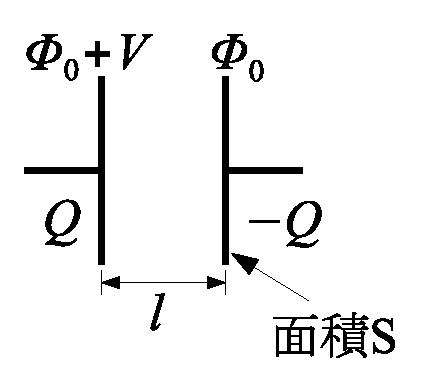
\includegraphics[width=50mm]{6.1.eps}
 \end{center}
 \caption{}
 \label{fig:one}
\end{figure}
\\
電気容量Cのコンデンサーについて式(2),(3)2通りの方法で静電エネルギーEを求める.
コンデンサーを2体とみなすと,式(2)から
\begin{eqnarray*}
\frac{1}{2}Q(\rho_0 + V) + \frac{1}{2}(-Q)\phi_0 = \frac{1}{2}QV = \frac{1}{2}CV^2
\end{eqnarray*}
電場の大きさは$|{\bf E}|=\frac{V}{l}$となるので,式(3)から
\begin{eqnarray*}
E = \frac{\varepsilon_0}{2} \int |{\bf E}|^2 dV 
= \frac{\varepsilon_0}{2} \left( \frac{V}{l} \right)^2 Sl = \frac{1}{2}\varepsilon_0 \frac{S}{l}V^2 = \frac{1}{2}CV^2
\end{eqnarray*}
\end{document}

